\section{Pitch Stability of an Vertically Open-loop Hopper}

\subsection{Jorge Cham's Dissertation - openloop control of 1DOF vertical hopper }
\begin{figure}[h]
\centering

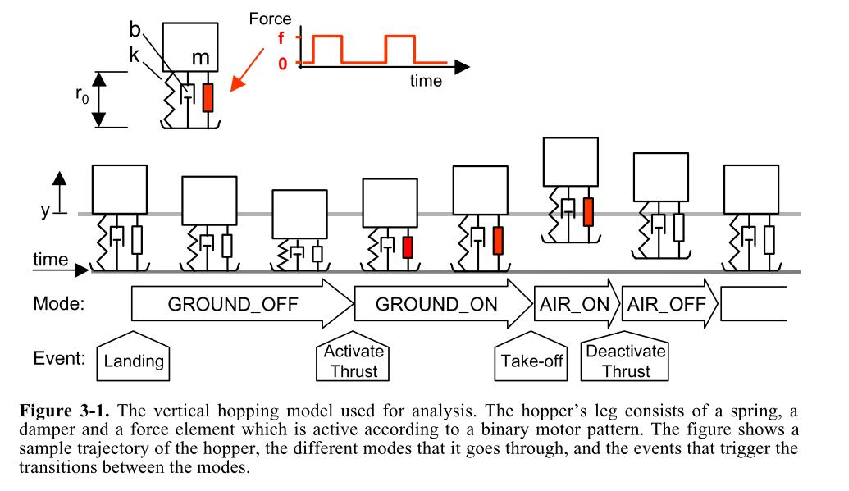
\includegraphics{test.pdf} 
\caption{The schematic of a 1 DOF hopper \cite{Cham2002}}
\label{fig.1DOF-Hopper}
\end{figure}


\subsubsection{Equation of motion}
Using the model as shown in Fig. \ref{fig.1DOF-Hopper}, during the stand phase (i.e. $y\leq 0$), the equation of motion can be expressed as:
\begin{align*}
m \ddot y = -b\dot y +-ky -mg + f
\end{align*}
\noindent where $m$ is the mass, $b$ is the damping, $k$ is the stiffness, $f$ is the control input.
Normalized by weight, the equation becomes
\begin{align*}
 \ddot y = -b/m\dot y +-k/my -g + f/m
\end{align*}

\noindent Expressed in state space form:

\begin{align}
\begin{bmatrix}
\dot y  \\
\ddot y 
\end{bmatrix} = \begin{bmatrix}
0 & 1 \\
-k/m & -b/m
\end{bmatrix}\begin{bmatrix}
 y  \\
\dot y 
\end{bmatrix} + 
\begin{bmatrix}
0  \\
-g+f/m 
\end{bmatrix}
\end{align}
or equivalently
\begin{align}
\label{eq:groundEOM}
\dot X = \begin{bmatrix}
0 & 1 \\
-\omega^2 & -2\xi\omega
\end{bmatrix}X + 
\begin{bmatrix}
0  \\
-g+f_n(t)
\end{bmatrix} &= \begin{bmatrix}
0 & 1 \\
-k_p & -k_d
\end{bmatrix}X + 
\begin{bmatrix}
0  \\
-g+f_n(t)
\end{bmatrix}
\end{align}
where $X \triangleq [y,\dot y]^T$.
When the hopper is in the air (i.e. $y> 0$, flight phase), 
\begin{align}
\label{eq:airEOM}
\dot X = \begin{bmatrix}
0 & 1 \\
0 & 0
\end{bmatrix}X + 
\begin{bmatrix}
0  \\
-g 
\end{bmatrix}
\end{align}
\noindent Define the force  of an open-loop motor pattern
\begin{align}
 f_n(t)=\begin{cases}
    f/m, & \text{if $t_{off}<t<t_{off}+t_{on}$}.\\
    0, & \text{otherwise}.
  \end{cases}
\end{align}

\begin{figure}[h]
	\centering
	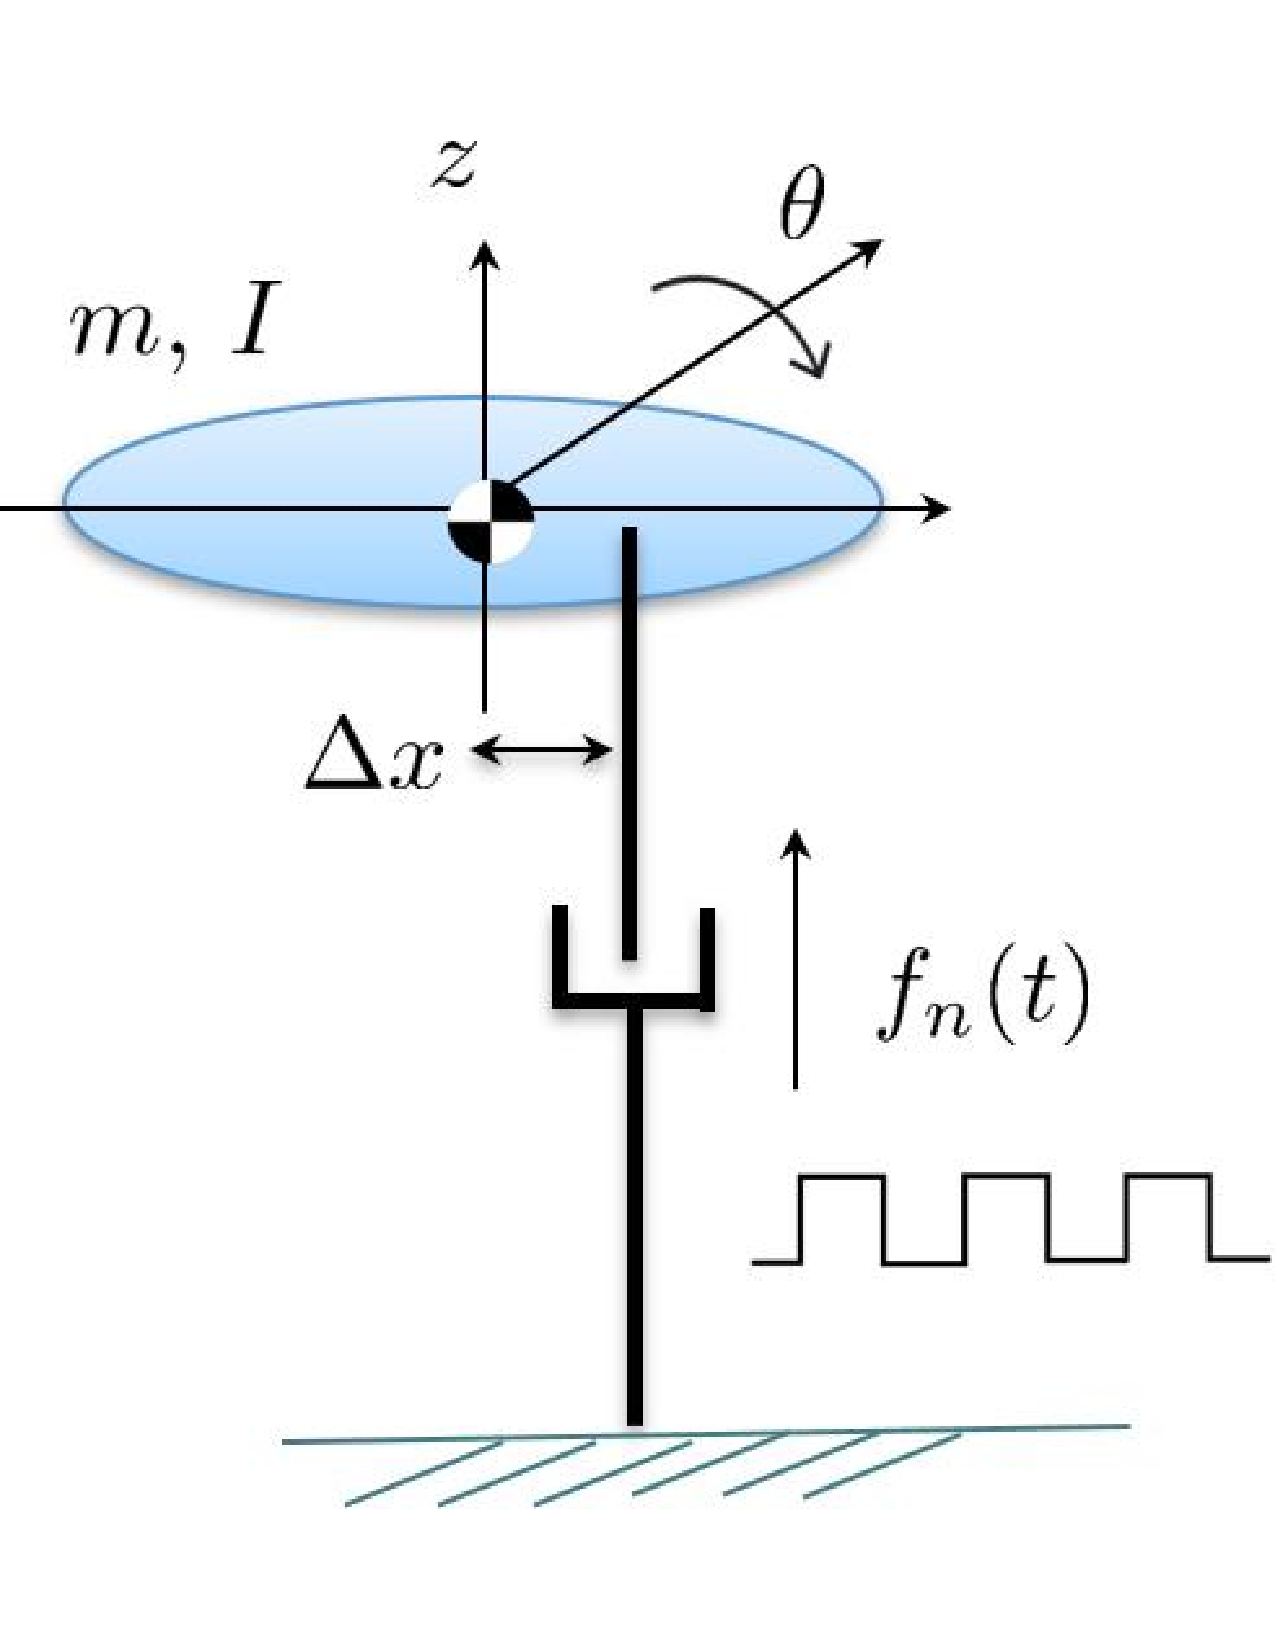
\includegraphics[scale = 0.2]{2DOF_Hopper.pdf} 
	\caption{The schematic of a 2 DOF hopper}
	\label{fig.2DOF-Hopper}
\end{figure}

\subsection{Stability Analysis of an Open-loop Controlled Hopper with Discrete Pitch Angle Control}
Use the state space of z motion form \ref{eq:groundEOM} with a simplified open-loop force input:

\begin{align}
\begin{bmatrix}
\dot z  \\
\ddot z 
\end{bmatrix} = \begin{bmatrix}
0 & 1 \\
-kp_z & -kd_z
\end{bmatrix}\begin{bmatrix}
 z  \\
\dot z 
\end{bmatrix} + 
\begin{bmatrix}
0  \\
-g+f_n(t)
\end{bmatrix}
\end{align}
where 
\begin{align}
 f_n(t)=\begin{cases}
    f_n\triangleq f/m, & \text{if $t_{flight}<t<t_{flight}+t_{contact}$}.\\
    0, & \text{otherwise}.
  \end{cases}
\end{align}
To further simplify the problem, assuming $f_n(t)$ is much more dominant than $-kp_zz-kd_z\dot z$-g so that:
\begin{align}
\label{eq:SimpleHopper}
\begin{bmatrix}
\dot z  \\
\ddot z 
\end{bmatrix} \approx \begin{bmatrix}
0 & 1 \\
0 & 0
\end{bmatrix}\begin{bmatrix}
 z  \\
\dot z 
\end{bmatrix} + 
\begin{bmatrix}
0  \\
f_n(t)
\end{bmatrix}
\end{align}
Assumptions:
\begin{itemize}
\item $f_n(t)$\footnote{Conceptually, the $f_n(t)$ can be treated as a force applied from a nonlinear component which connects the massless leg to the body (so there is no velocity change happen at foot strike)} can induce stable vertical hopping motion.
\item $t_0$ starts when the foot leaves the ground.
\item $t_{flight} + t_{contact} = T$, $t_{contact} = \alpha$, and $T>\alpha$
\end{itemize}
Then for the 2 DOF vertical hopper as shown in Fig. \ref{fig.2DOF-Hopper}, the pitch dynamics with feedback control can be expressed as:
\begin{align}
\begin{bmatrix}
\dot \theta  \\
\ddot \theta
\end{bmatrix} = \begin{bmatrix}
0 & 1 \\
0 & 0
\end{bmatrix}\begin{bmatrix}
 \theta  \\
\dot \theta
\end{bmatrix} + 
\begin{bmatrix}
0  \\
-f_n(t)m/I\Delta x
\end{bmatrix}
\end{align}
\subsubsection{Poincare Section}
\noindent Denote the state at the $n^{th}$ step Poincare section $\theta_n, \dot \theta_n$ (defined at the start of the flight phase). Then we can calculate the state at Poincare section at the $n+1^{th}$ step:
\begin{align}
\label{eq:PoincareSection1}
\dot \theta_{n+1} &= \dot \theta_{n} - \frac{f}{I}\Delta x t_{contact} \\
\nonumber\theta_{n_{touchDown}} &= \theta_{n} + \dot \theta_{n}t_{flight}\\
\nonumber\dot \theta_{n_{touchDown}} &= \dot \theta_{n}\\
\nonumber\theta_{n+1} &= \theta_{n} + \dot \theta_{n}t_{flight} + \dot \theta_{n}t_{contact} - \frac{1}{2}\frac{f}{I}\Delta xt^2_{contact}\\
\label{eq:PoincareSection2} & = \theta_n + T\dot \theta_n - \frac{1}{2}\frac{f}{I}\alpha^2\Delta x
\end{align}


\subsubsection{Poincare Map of Pitch Dynamics with Proportional Control}
By designing a proportional control such that $\Delta x = k\phi_n$ and defining $K =\frac{1}{2} \frac{f}{I}k$, Eq. \ref{eq:PoincareSection1} and Eq.\ref{eq:PoincareSection2} can be expressed as follows:
\begin{align*}
\theta_{n+1} &= \theta_n  - \alpha^2 K \theta_n + T\dot \theta_n\\
\dot \theta_{n+1} &= \dot \theta_n  - 2\alpha K \theta_n\\
\end{align*}
Arranged them in the state space equation, we can get a discrete map $M$ (i.e. Poincare Map, with set of difference equations):

\begin{align}
\label{eq:PoincareMap}
\begin{bmatrix}
\theta_{n+1}  \\
\dot \theta_{n+1}
\end{bmatrix} = \begin{bmatrix}
1-\alpha^2 K & T \\
-2\alpha K & 1
\end{bmatrix}\begin{bmatrix}
 \theta_n  \\
\dot \theta_n 
\end{bmatrix} = M
\begin{bmatrix}
 \theta_n  \\
\dot \theta_n 
\end{bmatrix}
\end{align}


\noindent \textbf{Eigen value analysis}\\
To analyze the stability of the equation in \ref{eq:PoincareMap}, we need to check whether the eigen values of Poincare map $M$ are within the unit cycle. Similar to the Rooth-Herwitz method for the continuous map, we can use Jury Stability Test (Ogata, 1985)\footnote{contents quotated from \cite{Cham2002}}, which states that a discrete system of two dimensions with the characteristic equations P(z) of the form:
\begin{align*}
P(z) = a_0z^2 + a_1z + a_2
\end{align*}
where $a_0>0$, is stable if the following conditions are all satisfied:
\begin{align*}
|a_2|&<a_0\\
a_0+a_1+a_2&>0\\
a_0-a_1+a_2&>0\\
|(a_0+a_2)(a_2-a_0)|&>|a_1(a_0-a_1)|\\
\end{align*}
For a Jacobian of the form 
\begin{align*}
J = \begin{bmatrix}
J_1 & J_2 \\
J_3 & J_4
\end{bmatrix}
\end{align*}
The characteristics equation can be expressed as follows:
\begin{align*}
P(z) = z^2-(J_1+J_4)z +(J_1J_4-J_2J_3)
\end{align*}
Substituting into the stable conditions stated above,
\begin{align}
\label{eq:condition1}
|(J_1J_4-J_2J_3)|&<1\\
\label{eq:condition2}
1-(J_1+J_4)+(J_1J_4-J_2J_3)&>0\\
\label{eq:condition3}
1+(J_1+J_4)+(J_1J_4-J_2J_3)&>0\\
\label{eq:condition4}
|(1+(J_1J_4-J_2J_3))((J_1J_4-J_2J_3)-1)|&>|(J_1+J_4)(1+(J_1+J_4)|
\end{align}

\noindent \textbf{Check condition Eq.\ref{eq:condition1}}:\\
First assuming $1-\alpha^2K+2T\alpha K>0$ 
\begin{align*}
1-\alpha^2K+2T\alpha K <1\\
\rightarrow -\alpha^2K+2T\alpha K < 0\\
\rightarrow \alpha K(-\alpha + 2T) < 0\\
\end{align*}
Since $\alpha>0$, $K>0$, and $T>\alpha$, the assumption cannot satisfy the condition.\\ Next, assuming $1-\alpha^2K+2T\alpha K<0$ :
\begin{align*}
1-\alpha^2K+2T\alpha K >-1\\
\rightarrow -1+\alpha^2K-2T\alpha K < 1\\
\rightarrow \alpha K(\alpha - 2T) < 2\\
\end{align*}
Since $T>\alpha$, the condition can always be satisfied, as long as the following condition is satisfied:
\begin{align*}
(J_1J_4-J_2J_3) = (1-\alpha^2K+2T\alpha K) <0
 \end{align*}
Combine conditions above we can get a new inequality as follows:
\begin{align}
\label{iq:detM}
-1< (J_1J_4-J_2J_3) = (1-\alpha^2K+2T\alpha K)  <0
 \end{align}


\noindent \textbf{Check condition Eq.\ref{eq:condition2}}:\\
\begin{align*}
1-(1-\alpha^2K+ 1) + (1-\alpha^2K+2T\alpha K)&>0\\
\rightarrow 2T\alpha K&>0 
\end{align*}
From the last inequality we can get the condition is \underline{always hold}.\\

\noindent \textbf{Check condition Eq.\ref{eq:condition3}}:\\
\begin{align*}
1  + (1-\alpha^2K+ 1) + (1-\alpha^2K+2T\alpha K) &>0 \\
\rightarrow 4-2 \alpha^2K+ 2T\alpha K &> 0\\
\rightarrow 4 + \alpha K(-2\alpha+ 2T) &> 0
\end{align*}
From the last inequality we can get the condition is \underline{always hold}.\\

\noindent \textbf{Check condition Eq.\ref{eq:condition4}}:\\
Based on Eq. \ref{iq:detM}, the left hand side of Eq. \ref{eq:condition4} can be rearranged as :
\begin{align*}
|(det(M)+1)(det(M)-1)| = |det(M)^2-1| = 1-det(M)^2
\end{align*}
From Eq. \ref{eq:condition2} and \ref{eq:condition3} we can got $(J_1+J_4)>0$, therefore the right hand side of Eq. \ref{eq:condition4} can be rearranged as:
\begin{align*}
|(J_1+J_4)(J_1+J_4 +1)| = (J_1+J_4)(J_1+J_4 +1)
\end{align*}
Therefore the Eq. \ref{eq:condition4} can be expressed as follows:
\begin{align*}
1-det(M)^2> tr(M) ( tr(M) + 1)
\end{align*}
where $det(M) = \prod\limits_{i}^{}\lambda_i = (J_1J_4-J_2J_3)$ is the determinant of matrix $M$ and $tr(M)=\sum\limits_{i}^{}\lambda_i = (J_1 + J_4)$ is the trace of the matrix $M$.\\

\noindent \textbf{To sum up}\\
For the (Poincare) stability, the following conditions need to be satisfied:
\begin{align}
-1<det(M)&<0\\
0< tr(M) ( tr(M) + 1)&<1-det(M)^2
\end{align}
where
\begin{align*}
det(M) &= 1- \alpha^2K + 2T\alpha K\\
tr(M) &= 2- \alpha^2K \\
K &= \frac{1}{2}\frac{f_n}{I}k
\end{align*}

\noindent \textbf{Result}\\
After check the sign of the $det(M)$, it was found that $det(M)$ always $>0$:
\begin{align*}
 1-\alpha^2K+2T\alpha K = 1 + \alpha K(-\alpha+2T)>0
\end{align*}
Therefore, it is concluded that proportional control with this system setup cannot stablize the pitch dynamics.
\pagebreak

\subsubsection{Poincare Map of Pitch Dynamics with PD Control}
By designing a PD control such that $\Delta x = k_p\theta_n+k_d\dot \theta_n$ and defining $K =\frac{1}{2} \frac{f}{I}k_p$, $C =\frac{1}{2} \frac{f}{I}k_d$, Eq. \ref{eq:PoincareSection1} and Eq.\ref{eq:PoincareSection2} can be expressed as follows:
\begin{align*}
\theta_{n+1} &= \theta_n  - \alpha^2 K \theta_n + T\dot \theta_n - \alpha^2 C \dot\theta_n\\
\dot \theta_{n+1} &= \dot \theta_n  - 2\alpha K \theta_n- 2\alpha C \dot\theta_n\\
\end{align*}
Arranged them in the state space equation, we can get a discrete map $M_{pd}$:

\begin{align}
\label{eq:PoincareMapPD}
\begin{bmatrix}
\theta_{n+1}  \\
\dot \theta_{n+1}
\end{bmatrix} = \begin{bmatrix}
1-\alpha^2 K & T-\alpha^2 C \\
-2\alpha K & 1-2\alpha C
\end{bmatrix}\begin{bmatrix}
 \theta_n  \\
\dot \theta_n 
\end{bmatrix} = M_{pd}
\begin{bmatrix}
 \theta_n  \\
\dot \theta_n 
\end{bmatrix}
\end{align}






%\begin{align*}
%\begin{bmatrix}
%\theta_{n+1}  \\
%\sqrt\alpha\dot \phi_{n+1}
%\end{bmatrix} = \begin{bmatrix}
%1-2\alpha K & 1 \\
%-\sqrt{\alpha}K & \sqrt\alpha
%\end{bmatrix}\begin{bmatrix}
% \theta_n  \\
% \dot \phi_n 
%\end{bmatrix} \rightarrow
%\end{align*}

%\begin{align}
%\begin{bmatrix}
%\theta_{n+1}  \\
%\dot \phi_{n+1}
%\end{bmatrix} = \begin{bmatrix}
%1-2\alpha K & 1 \\
%-K & 1
%\end{bmatrix}\begin{bmatrix}
% \theta_n  \\
%\dot \phi_n 
%\end{bmatrix}
%\end{align}


\pagebreak
\subsubsection{Analytical Solution for Eq.\ref{eq:SimpleHopper}}
Start from $t_0$ (the beginning of the flight phase), assuming $Z = [0, \dot z_0]^T$, then we can get:

\begin{align}
z(t_{flight}) &= \dot z_0t_{flight} - 1/2gt^2_{flight} = 0\\
\dot z(t_{flight}) &= \dot z_0 - gt_{flight} = -\dot z_0
\end{align}
where a constraint for the $\dot z_0$ can be derived:
\begin{align}
\label{eq:tFlight}
\dot z_0 =  1/2gt_{flight}\\
\end{align}
Then we can derive the solution at the end of the touch down:
\begin{align}
z(1) &= -\dot z_0t_{contact} + (f/m -g)t_{contact}^2 = 0 \\
\dot z(1) &= -\dot z_0 + (f/m -g)t_{contact} = \dot z_0
\end{align}
where another constraint for the $\dot z_0$ can be derived:
\begin{align}
\label{eq:tContact}
\dot z_0 =  1/2(f/m-g)t_{contact}
\end{align}

\noindent \textbf{Period $T$, contact force $f$ and $t_{contact}$ are dependent }
From Eqs. \ref{eq:tContact} and \ref{eq:tFlight} we can get

\begin{align*}
1/2gt_{flight} &=  1/2(f/m-g)t_{contact}\\
\rightarrow t_{flight} &= (f/mg -1) t_{contact}\\
\rightarrow t_{flight} + t_{contact} &= T = (f/mg)t_{contact}
\end{align*}

\pagebreak	


\subsection{Stability Analysis of an Open-loop Controlled Hopper with Continuous Pitch Angle Control}
Consider the case that $\Delta x = k\theta(t)$ or $\Delta x = k_p\theta(t) + k_d\dot\theta(t)$, then the pitch angle will be controlled continuously in the stance phase. 

%The flight phase remained the same as there is no ground reaction force can act on the body: 
%\begin{align}
%\label{eq:EOM_flight}
%\dot X = 
%\begin{bmatrix}
%\dot \theta  \\
%\ddot \theta
%\end{bmatrix} = \begin{bmatrix}
%0 & 1 \\
%0 & 0
%\end{bmatrix}\begin{bmatrix}
%\theta \\
%\dot \theta
%\end{bmatrix}
%\end{align}

\subsubsection{Poincare map of Hopper with Continuous Proportional Control}

Assuming $\Delta x = k\theta(t)$, then the system dynamic in the stance phase becomes:
\begin{align}
\label{eq:EOM_flight2}
\dot X = 
\begin{bmatrix}
\dot \theta  \\
\ddot \theta
\end{bmatrix} = \begin{bmatrix}
0 & 1 \\
-k\frac{f}{I} & 0
\end{bmatrix}X \triangleq \begin{bmatrix}
0 & 1 \\
-2K & 0
\end{bmatrix}X = AX
\end{align}
\noindent where $K =\frac{1}{2} \frac{f}{I}k$. Again denoting the state at the $n^{th}$ step Poincare section $X_n = [\theta_n, \dot \theta_n]^T$ (defined at the start of the flight phase). Then we can first calculate the touchdown state at $n_{th}$ step:
\begin{align}
\nonumber\theta_{n_{TD}} &= \theta_{n} + \dot \theta_{n}t_{flight}\\
\nonumber\dot \theta_{n_{TD}} &= \dot \theta_{n}
\end{align}
and $X_{n_{TD}} = [\theta_{n_{TD}}, \dot \theta_{n_{TD}}]^T$ then can be expressed as:
\begin{align}
X_{n_{TD}} = \begin{bmatrix}
        1 & (T-\alpha) \\
        0 & 1
        \end{bmatrix}X_n
\end{align}
Next, assuming the contact time is exactly $t_{contact}= \alpha$ (e.g. no perturbation in $z$ direction), then the $X_{n+1} = [\theta_{n+1}, \dot \theta_{n+1}]^T$ can be expressed with $X_{n_{TD}} = [\theta_{n_{TD}}, \dot \theta_{n_{TD}}]^T$:
\begin{align}
X_{n+1} &= e^{A\alpha}(X_{n{TD}} - X_{eq}) +X_{eq} \\
        &= e^{A\alpha}(\begin{bmatrix}
        1 & (T-\alpha) \\
        0 & 1
        \end{bmatrix}X_n -X_{eq}) + X_{eq}
\end{align}
where $X_{eq} = [0,0]^T$ is the equilibrium point of Eq. \ref{eq:EOM_flight2}. Therefore, we can get the Poincare map in this case is:
\begin{align}
M &=   e^{A\alpha}(\begin{bmatrix}
        1 & (T-\alpha) \\
        0 & 1
        \end{bmatrix}
\end{align}

\noindent Using symbolic tool in MATLAB, we can derive the closed-form expression of $M$ as follows:

\begin{align*}
M =& \begin{bmatrix}
M_{11} M_{12}  \\
M_{21} M_{22}
\end{bmatrix}\\
\end{align*}
where
\begin{align*}
M_{11} =&\frac{{\mathrm{e}}^{\sqrt{2}\,\sqrt{-K}\,a}}{2}+\frac{{\mathrm{e}}^{-\sqrt{2}\,\sqrt{-K}\,a}}{2}\\
M_{12} =&\left(\frac{{\mathrm{e}}^{\sqrt{2}\,\sqrt{-K}\,a}}{2}+\frac{{\mathrm{e}}^{-\sqrt{2}\,\sqrt{-K}\,a}}{2}\right)\,\left(T-a\right)+\frac{\sqrt{2}\,{\mathrm{e}}^{\sqrt{2}\,\sqrt{-K}\,a}-\sqrt{2}\,{\mathrm{e}}^{-\sqrt{2}\,\sqrt{-K}\,a}}{4\,\sqrt{-K}}\\
M_{21} =&\frac{\sqrt{2}\,\sqrt{-K}\,{\mathrm{e}}^{\sqrt{2}\,\sqrt{-K}\,a}}{2}-\frac{\sqrt{2}\,\sqrt{-K}\,{\mathrm{e}}^{-\sqrt{2}\,\sqrt{-K}\,a}}{2}\\
M_{22} =&\frac{{\mathrm{e}}^{\sqrt{2}\,\sqrt{-K}\,a}}{2}+\frac{{\mathrm{e}}^{-\sqrt{2}\,\sqrt{-K}\,a}}{2}+\left(\frac{\sqrt{2}\,\sqrt{-K}\,{\mathrm{e}}^{\sqrt{2}\,\sqrt{-K}\,a}}{2}-\frac{\sqrt{2}\,\sqrt{-K}\,{\mathrm{e}}^{-\sqrt{2}\,\sqrt{-K}\,a}}{2}\right)\,\left(T-a\right)
\end{align*}


\subsubsection{Poincare Map of Hopper with Continuous PD Control}

Assuming $\Delta x = k_p\theta(t) + k_d\dot\theta(t)$, then the system dynamic in the stance phase becomes:
\begin{align}
\label{eq:EOM_flight3}
\dot X = 
\begin{bmatrix}
\dot \theta  \\
\ddot \theta
\end{bmatrix} &= \begin{bmatrix}
0 & 1 \\
-k_p\frac{f}{I} & -k_d\frac{f}{I}
\end{bmatrix}X \triangleq \begin{bmatrix}
0 & 1 \\
-2K & -2C
\end{bmatrix}X = AX\\
M_{pd} &=   e^{A\alpha}(\begin{bmatrix}
        1 & (T-\alpha) \\
        0 & 1
        \end{bmatrix}
\end{align}

\noindent Using symbolic tool in MATLAB, we can derive the closed-form expression of $M_{pd}$ as follows:

\begin{align*}
M_{pd} =& \begin{bmatrix}
M_{11} M_{12}  \\
M_{21} M_{22}
\end{bmatrix}\\
\end{align*}
where
\begin{align*}
M_{11} =& \frac{C\,{\mathrm{e}}^{a\,\sqrt{C^2-2\,K}-C\,a}-C\,{\mathrm{e}}^{-C\,a-a\,\sqrt{C^2-2\,K}}+{\mathrm{e}}^{a\,\sqrt{C^2-2\,K}-C\,a}\,\sqrt{C^2-2\,K}+{\mathrm{e}}^{-C\,a-a\,\sqrt{C^2-2\,K}}\,\sqrt{C^2-2\,K}}{2\,\sqrt{C^2-2\,K}}\\
M_{12} =& 
\frac{{\mathrm{e}}^{a\,\sqrt{C^2-2\,K}-C\,a}-{\mathrm{e}}^{-C\,a-a\,\sqrt{C^2-2\,K}}}{2\,\sqrt{C^2-2\,K}}+\\ &\frac{\left(T-a\right)\,\left(C\,{\mathrm{e}}^{a\,\sqrt{C^2-2\,K}-C\,a}-C\,{\mathrm{e}}^{-C\,a-a\,\sqrt{C^2-2\,K}}+{\mathrm{e}}^{a\,\sqrt{C^2-2\,K}-C\,a}\,\sqrt{C^2-2\,K}+{\mathrm{e}}^{-C\,a-a\,\sqrt{C^2-2\,K}}\,\sqrt{C^2-2\,K}\right)}{2\,\sqrt{C^2-2\,K}}\\
M_{21} =& -\frac{K\,{\mathrm{e}}^{a\,\sqrt{C^2-2\,K}-C\,a}-K\,{\mathrm{e}}^{-C\,a-a\,\sqrt{C^2-2\,K}}}{\sqrt{C^2-2\,K}}\\
M_{22} =& \frac{C\,{\mathrm{e}}^{-C\,a-a\,\sqrt{C^2-2\,K}}-C\,{\mathrm{e}}^{a\,\sqrt{C^2-2\,K}-C\,a}+{\mathrm{e}}^{a\,\sqrt{C^2-2\,K}-C\,a}\,\sqrt{C^2-2\,K}+{\mathrm{e}}^{-C\,a-a\,\sqrt{C^2-2\,K}}\,\sqrt{C^2-2\,K}}{2\,\sqrt{C^2-2\,K}}-
\\ &\frac{\left(T-a\right)\,\left(K\,{\mathrm{e}}^{a\,\sqrt{C^2-2\,K}-C\,a}-K\,{\mathrm{e}}^{-C\,a-a\,\sqrt{C^2-2\,K}}\right)}{\sqrt{C^2-2\,K}}
\end{align*}


\pagebreak

\subsubsection{General Solution of Poincare Map of Hybrid Linear Systems}


\begin{align}
\dot Z = AZ +B
\end{align}
where \textbf{A is invertible}. If the \textbf{mode transistion  is time-based}, then we can augment the state of the system with $t$:
\begin{align}
\label{eq:AtEOM}
\dot X = 
\begin{bmatrix}
\dot t  \\
\dot Z
\end{bmatrix} = \begin{bmatrix}
0 & 0 \\
0 & A
\end{bmatrix}X + \begin{bmatrix}
1\\%
B 
\end{bmatrix}
\end{align}
where $X = [t,Z]^T$. Assuming the mode trasition happened under the following condition:
\begin{align}
e^T X = 0
\end{align}
and takes time $\Delta t$ from $X_n$ to $X_{n+1}$, then the Poincare map (Jacobian matrix) can be expressed as:
\begin{align}
\frac{\partial  X_{n+1}}{\partial  X_{n}} = -\dot X_{n+1}(e^T\dot X_{n+1})^{-1} e^T\begin{bmatrix}
1 & 0 \\
0 & e^{A\Delta t}
\end{bmatrix} + 
\begin{bmatrix}
1 & 0 \\
0 & e^{A\Delta t}
\end{bmatrix}
\end{align}




\pagebreak